\documentclass[bwprint]{gmcmthesis}
\usepackage[framemethod=TikZ]{mdframed}
\title{高压油管稳定控压策略的研究}
\baominghao{111} %参赛队号
\schoolname{浙江大学}%学校名称
\membera{葛明阳} %队员A
\memberb{郑欣怡} %队员B
\memberc{董萌苇} %队员C
\begin{document}

 %生成标题
 \maketitle

 %填写摘要
\begin{abstract}
本文对高压油管、高压油泵和喷嘴口建立\textbf{微分模型},通过数值解法得到高压油管的油压变化,并通过设定优化目标,建立规划问题。使用\textbf{优先搜索、控制变量、稀疏遍历}等算法提高求解问题的速度与精度。同时,也对模型中主要参数进行了灵敏度分析,将主要参数设置到合适的数值。
\keywords{微分方程;Runge-Kutta; 非线性规划; 优先搜索; 稀疏遍历; 迭代逼近}

\end{abstract}

\pagestyle{plain}

%目录 不推荐加
%\tableofcontents

\section{问题重述}
信号干扰下的超宽带(UWB)精确定位问题,是指考虑\textbf{信号干扰}的前提下,利用基于飞行时间(Time of Flignt,TOF)测距原理的UWB定位技术,采集锚点(anchor)与靶点(Tag)之间的距离,确定Tag的精确定位(3维坐标)。

\textbf{任务1},对在场景1:$5000mm*3000mm*3000mm$测试环境范围内324个不同位置Tag,分别在信号干扰和信号无干扰下接收4个角落anchor信号,所解算出的距离数据文件,考虑在同一位置连续时间中自动采集多组数据、采集异常等问题,进行数据预处理,最终对每个位置Tag只保留有效采集的信号干扰和信号无干扰下各一组数据。

\textbf{任务2},分别利用经任务1处理的信号无干扰下的“正常数据”和信号干扰下的“异常数据”,求解各个位置Tag的精确定位(3维坐标)。

\textbf{任务3},对在场景2:$5000mm*3000mm*3000mm$测试环境范围内,5个Tag在信号干扰、5个Tag在信号无干扰下接收4个位置anchor信号,所解算出的距离数据,求解相应位置Tag的精确定位(3维坐标)。

\textbf{任务4},提出一种判断数据是在信号有无干扰的情况下采集的方法,并使用场景1经任务1处理后的数据和场景2数据进行验证。

\textbf{任务5},根据一段时间内连续采集动态靶点的多组数据,判断各组数据是在信号有无干扰的情况下采集,并分别求解相应Tag的精确定位,结合靶点自身运动规律画出运动轨迹。

\subsection{引言}
创意平板折叠桌注重于表达木制品的优雅和设计师所想要强调的自动化与功能性。为了增大有效使用面积。设计师以长方形木板的宽为直径截取了一个圆形作为桌面,又将木板剩余的面积切割成了若干个长短不一的木条,每根木条的长度为平板宽到圆上一点的距离,分别用两根钢筋贯穿两侧的木条,使用者只需提起木板的两侧,便可以在重力的作用下达到自动升起的效果,相互对称的木条宛如下垂的桌布,精密的制作工艺配以质朴的木材,让这件工艺品看起来就像是工业革命时期的机器。

\subsection{问题的提出}

\subsubsection{问题的提出内容一}

(1) 围绕创意平板折叠桌的动态变化过程、设计加工参数,本文依次提出如下问题:
给定长方形平板尺寸 ($120 cm \times 50 cm \times 3 cm$),每根木条宽度(2.5cm),连接桌腿木条的钢筋的位置,折叠后桌子的高度(53 cm)。要求建立模型描述此折叠桌的动态变化过程,并在此基础上给出此折叠桌的设计加工参数和桌脚边缘线的数学描述。

(2)折叠桌的设计应做到产品稳固性好、加工方便、用材最少。对于任意给定的折叠桌高度和圆形桌面直径的设计要求,讨论长方形平板材料和折叠桌的最优设计加工参数,例如,平板尺寸、钢筋位置、开槽长度等。对于桌高70 cm,桌面直径80 cm的情形,确定最优设计加工参数。

(3)给出软件设计的数学模型,可以根据客户任意设定的折叠桌高度、桌面边缘线的形状大小和桌脚边缘线的大致形状,给出所需平板材料的形状尺寸和切实可行的最优设计加工参数,使得生产的折叠桌尽可能接近客户所期望的形状,并根据所建立的模型给出几个设计的创意平板折叠桌。要求给出相应的设计加工参数,画出至少8张动态变化过程的示意图。

\section{模型的假设}

\begin{itemize}
\item 忽略实际加工误差对设计的影响;
\item 木条与圆桌面之间的交接处缝隙较小,可忽略;
\item 钢筋强度足够大,不弯曲;
\item 假设地面平整。
\end{itemize}

\section{符号说明}

\begin{tabular}{ccc}
 \hline
 \makebox[0.25\textwidth][c]{符号}	&  \makebox[0.25\textwidth][c]{意义} &\makebox[0.25\textwidth][c]{单位}\\ \hline
 D    & 木条宽度(cm)   &cm\\ \hline
 L   & 木板长度(cm)	 &cm \\ \hline
 W   & 木板宽度(cm)	 &cm \\ \hline
 N	    & 第n根木条	   &cm \\ \hline
 T	    & 木条根数	   &cm \\ \hline
 H	    & 桌子高度(cm)	 &cm \\ \hline
 R	    & 桌子半径(cm)	  &cm\\ \hline
 R	    & 桌子直径(cm)	 &cm \\ \hline
\end{tabular}

\begin{tabular}{ccc}
    
    
\end{tabular}
\section{问题qqQQAAAAaaaAAAAAAAAAAAAAAAAA}
\section{问题分析}

\subsection{问题一分析}
题目要求建立模型描述折叠桌的动态变化图,由于在折叠时用力大小的不同,我们不能描述在某一时刻折叠桌的具体形态,但我们可以用每根木条的角度变化来描述折叠桌的动态变化。首先,我们知道折叠桌前后左右对称,我们可以运用几何知识求出四分之一木条的角度变化。最后,根据初始时刻和最终形态两种状态求出桌腿木条开槽的长度。
$$\pi\times$$
\begin{equation}
\pi\times
\end{equation}


\subsection{问题二分析}
题目要求从折叠桌的稳固性好、加工方便、用材最少三个角度,确定设计加工参数。我们可以从应力、支撑面积考虑稳固性,从开槽长度考虑加工方便,从木板长度考虑用材最少。而它们之间又是相互制约,我们需要确定最优设计加工参数,可以建立非线性规划模型,用lingo软件来求解最优设计加工参数(平板尺寸、钢筋位置、开槽长度等),这里以合力的方向(斜向上)与最长木条(桌腿)的夹角方向最小为目标函数,以木条所承受应力小于木条的许用应力、支撑面积大于桌面面积、木条的开槽长度小于木条本身长为约束条件。
\begin{figure}[b]
\centering
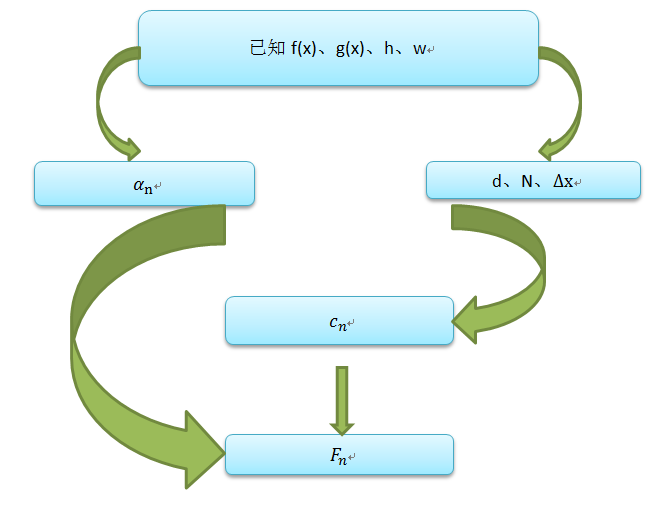
\includegraphics[width=.7\textwidth]{1.png}
\caption{问题三流程图}
\end{figure}
\subsection{问题三分析}
题目要求制作软件的意思就是客户给定折叠桌高度、桌面边缘线的形状大小和桌脚边缘线的大致形状,将这些信息输入程序就得到客户想要的桌子。我们在求解最优设计加工参数时,自行给定桌面边缘线形状(椭圆、相交圆等),桌脚边缘线形状,折叠桌高度,应用第二问的非线性规划模型,用MATLAB软件绘制折叠桌截面图,得到自己设计的创意平板折叠桌。



%参考文献   手工录入
%\begin{thebibliography}{9}%宽度9
% \bibitem{bib:one} ....
% \bibitem{bib:two} ....
%\end{thebibliography}

%采用bibtex方案
\cite{mittelbach_latex_2004,wright_latex3_2009,beeton_unicode_2008,vieth_experiences_2009}

\bibliographystyle{gmcm}
\bibliography{example}


\newpage
%附录
\appendix
%\setcounter{page}{1} %如果需要可以自行重置页码。
\section{我的 MATLAB 源程序}
\begin{lstlisting}[language=Matlab]%设置不同语言即可。
kk=2;[mdd,ndd]=size(dd);
while ~isempty(V)
[tmpd,j]=min(W(i,V));tmpj=V(j);
for k=2:ndd
[tmp1,jj]=min(dd(1,k)+W(dd(2,k),V));
tmp2=V(jj);tt(k-1,:)=[tmp1,tmp2,jj];
end
tmp=[tmpd,tmpj,j;tt];[tmp3,tmp4]=min(tmp(:,1));
if tmp3==tmpd, ss(1:2,kk)=[i;tmp(tmp4,2)];
else,tmp5=find(ss(:,tmp4)~=0);tmp6=length(tmp5);
if dd(2,tmp4)==ss(tmp6,tmp4)
ss(1:tmp6+1,kk)=[ss(tmp5,tmp4);tmp(tmp4,2)];
else, ss(1:3,kk)=[i;dd(2,tmp4);tmp(tmp4,2)];
end;end
dd=[dd,[tmp3;tmp(tmp4,2)]];V(tmp(tmp4,3))=[];
[mdd,ndd]=size(dd);kk=kk+1;
end; S=ss; D=dd(1,:);
 \end{lstlisting}
\end{document} 